\chapter{Noise Analysis}

 \section{Introduction}
 This chapter gives a comprehensive account of the testing which was done on the completed DWL system to account for the various sources of noise. The purpose of the noise analysis is to quantify the noise observed in the system and attribute it to the appropriate sources, while investigating how component, architecture, and operating point choice affects this. This chapter is separate from the functional testing of \autoref{sec:functionalAnalysis}, as the experimental setup differs significantly, and the results from these experiments will indeed be used to inform the expected results of the experiments in \autoref{sec:functionalAnalysis}, and to construct an optimal experimental setup in those cases.

 \section{A: Electronic and Shot Noise}
 
 \subsection{Experimental Goals}
 As discussed in \autoref{sec:lit-noiseSources}, a coherent DWL performs best when it is
 shot-noise limited: the shot noise of the local oscillator (LO) must dominate every other
 noise source at the detector. Experiment A characterises the receiver's noise floor with
 the LO as the only light on the detector, so that the individual noise contributions can be
 separated and measured. It has the following goals:
 
 \begin{itemize}
 	\item \textbf{Measure the electronic noise floor (A1).} With the laser off, measure the
 	noise of the PD100B and acquisition chain alone, and compare it with the input-referred
 	noise specified in the PD100B datasheet. Agreement with the datasheet validates the
 	data collection and post-processing chain used in all later experiments.
 	
 	\item \textbf{Measure shot noise as a function of LO power (A2).} Step the laser drive
 	current to vary the LO power reaching the balanced detector, and confirm that the excess
 	noise above the electronic floor grows linearly with LO power, as expected for shot noise.
 	
 	\item \textbf{Choose the operating point.} From the A2 results, find the LO power at which
 	shot noise overtakes the electronic floor, and choose a laser operating point at which the
 	system is close enough to the shot-noise limit to meet requirement P2
 	(\autoref{tab:requirements}).
 	
 	\item \textbf{Quantify RIN and validate balanced detection (A3).} Repeat the measurement
 	with only one photodiode connected, making the PD100B a single-ended detector. Comparing
 	this with the balanced case measures the laser's relative intensity noise (RIN) and
 	confirms that the balanced detector cancels this common-mode noise as intended. This experiment is only included for completeness, to demonstrate RIN cancellation, and the results are given in Appendix \ref{appendix:RINValidation}.
 \end{itemize} 

 \subsection{Experimental Methodology}
 The experimental setup used is given in \autoref{fig:expASetup}:

 \begin{figure}[H]
 \resizebox{\textwidth}{!}{%
     \centering
 \begin{tikzpicture}[
     font=\small,
     >={Stealth[length=2.2mm]},
     block/.style={draw, rounded corners=2pt, minimum height=1.3cm,
                   minimum width=3.0cm, align=center, inner sep=4pt,
                   fill=white},
     subblock/.style={block, minimum width=2.6cm, minimum height=1.1cm},
     fibre/.style={->, thick},
     elec/.style={->, thick, gray},
     lbl/.style={font=\scriptsize, midway},
     portcap/.style={draw, fill=black, minimum width=1.6mm, minimum height=3.2mm,
                 inner sep=0pt},
   ]
 
   % ======================= laser source (sub-blocks) =======================
   \node[subblock] (drv) at (0,0.95)
     {Laser driver\\[-1pt]{\scriptsize\itshape Koheron DRV200S}};
   \node[subblock] (tec) at (0,-0.95)
     {TEC controller\\[-1pt]{\scriptsize\itshape Koheron TEC100L}};
   \node[subblock, minimum height=3.0cm] (diode) at (4.9,0)
     {1550\,nm DFB\\laser diode\\[2pt]
      {\scriptsize\itshape BFLD-1550-20SM}\\[-2pt]{\scriptsize\itshape in Koheron}\\[-2pt]{\scriptsize\itshape BTF100D mount}};
 
   \draw[elec] (drv.east) -- node[lbl, above, align=center] {current\\[-2pt](swept)}
                  (drv.east -| diode.west);
   \draw[elec, <->] (tec.east) -- node[lbl, above, align=center] {TEC /\\[-2pt]thermistor}
                   (tec.east -| diode.west);
 
   \begin{scope}[on background layer]
     \node[draw, rounded corners=4pt, dashed, inner sep=8pt, fill=gray!6,
           fit=(drv)(tec)(diode), label={[font=\small]above:Laser source}] (src) {};
   \end{scope}
 
   % ======================= optical path =======================
   \node[block, right=3.0cm of src.east |- diode.east, anchor=west] (split)
     {90:10 fibre\\splitter};
 
   % 90 % port capped
   \coordinate (capat) at ($(split.north east)+(2.4,1.3)$);
   \node[portcap] (capnode) at (capat) {};
   \node[right=2pt of capnode, font=\scriptsize, align=left]
     {90\,\% port capped\\[-2pt](FC/APC dust cap)};
 
   \node[block, right=2.6cm of split] (mix)
     {50:50 fibre\\coupler};
 
   % unused coupler input
   \coordinate (unused) at ($([yshift=-3mm]mix.west)+(-1.1,0)$);
   \node[portcap] (capin) at (unused) {};
   \node[below=1pt of capin, font=\scriptsize, align=center] {input 2\\[-2pt]unused};
 
   \node[block, right=2.2cm of mix] (pd)
     {Balanced detector\\[-1pt]{\scriptsize\itshape Koheron PD100B}\\[-3pt]{\scriptsize\itshape 39\,kV/A, 100\,MHz}};
   \node[block, right=1.9cm of pd] (scope)
     {Oscilloscope\\[-1pt]{\scriptsize\itshape Keysight EDUX1002G}};
   \node[block, below=1.2cm of scope] (pc)
     {PC\\[-1pt]{\scriptsize\itshape Python acquisition,}\\[-3pt]{\scriptsize\itshape Welch PSD analysis}};
 
   % ======================= connections =======================
   \draw[fibre] (diode.east) -- node[lbl, above, align=center]
       {laser output\\[-2pt]1550\,nm, 20\,mW}
       node[lbl, below] {SM fibre, FC/APC} (split.west);
 
   \draw[fibre] ([xshift=-6mm]split.north east) |- node[lbl, pos=0.75, above] {90\,\%}
       (capnode.west);
 
   \draw[fibre] ([yshift=3mm]split.east) -- node[lbl, above] {10\,\% (LO)}
       ([yshift=3mm]mix.west);
   \draw[thick] (capin.east) -- ([yshift=-3mm]mix.west);
 
   % coupler outputs -> detector
   \draw[fibre] ([yshift=3mm]mix.east) -- node[lbl, above] {output 1}
       ([yshift=3mm]pd.west);
   \draw[fibre] ([yshift=-3mm]mix.east) -- node[pos=0.5, font=\Large,
       red!75!black] (brk) {$\times$} ([yshift=-3mm]pd.west);
   \node[below=4pt of brk, font=\scriptsize, align=center, red!75!black]
     {output 2 disconnected\\[-2pt]for unbalanced (A3)};
 
   % detection chain
   \draw[elec] (pd) -- node[lbl, above] {PD out} node[lbl, below] {SMA--BNC} (scope);
   \draw[elec] (scope) -- node[lbl, right] {USB} (pc);
 
  
 
   % ======================= legend =======================
   \begin{scope}[shift={(src.west |- pc.south)}, yshift=-0.2cm]
     \draw[fibre] (0,0) -- (0.9,0);
     \node[right, font=\scriptsize] at (0.9,0) {optical fibre (single-mode, FC/APC)};
     \draw[elec] (6.2,0) -- (7.1,0);
     \node[right, font=\scriptsize] at (7.1,0) {electrical};
     \node[portcap] at (9.6,0) {};
     \node[right, font=\scriptsize] at (9.7,0) {capped / unused port};
   \end{scope}
 \end{tikzpicture}}
 \caption{Experimental setup A}
     \label{fig:expASetup}
 \end{figure}

 It can be seen that this differs from the full system setup. The circulator and collimator are unused for this experiment. The 90\% splitter arm is left unconnected and is capped. Only the 10\% splitter arm (LO) is connected to the one arm of the 50:50 coupler. Both outputs of the coupler are connected to the balanced detector, except in the case of experiment A3. Since there is no circulator, collimator or target, the only light reaching the detector is the LO itself. With no second optical field there is no beat term (as in \autoref{eqn:beatSignal}), and the LO contributes only a DC photocurrent, which is removed by the detector's AC coupling. Thus, the signal at the detector will be a pure noise signal, containing only electronic noise and shot noise. Note that phase-induced intensity noise is not present here, as it originates from reflections in the collimator and circulator which are not present in this setup, and RIN is assumed to be cancelled fully by balanced detection.

 The experiment is divided into three phases, with slightly different configurations for each in order to give different measurands, as shown in \autoref{tab:expAParts}:

 \begin{table}[H]
     \centering
     \begin{tabular}{|p{3.5cm}|p{7cm}|p{5cm}|}
     \hline
         \textbf{ID} & \textbf{Configuration} & \textbf{Quantity Measured} \\ \hline
          A1 & Laser output off, detector switched on & Electronic noise only \\ \hline
          A2 & Laser output on (current varied), detector switched on, both detector inputs connected & Electronic noise + shot noise \\ \hline
          A3 (supplementary experiment) & Laser output on (current varied), detector switched on, only one detector input connected & Electronic noise + shot noise + full RIN \\ \hline
     \end{tabular}
     \caption{Experiment A phases and configurations}
     \label{tab:expAParts}
 \end{table}

 For each measurement, the laser is held at a fixed drive current and
 100 records of the detector output are captured sequentially with the oscilloscope and
 transferred to a laptop. Each record contains 25\,000 samples at 125\,MSa/s (200\,$\mu$s).
 A1 requires only a single measurement, while A2 and A3 are repeated over a range of drive
 currents up to the 48\,mA operating point.
 
 The PSD of each record is estimated using Welch's method (Hann window, 2\,500-sample
 segments with 50\,\% overlap, giving a 50\,kHz resolution) rather than a single periodogram,
 since averaging over segments greatly reduces the variance of the estimate, giving a smoother curve. Because the noise
 is stationary (properties don't change across records), the PSDs of the 100 records can then be averaged as well for further smoothing.
 
 To compare the results with a single figure, the PSD can be averaged over the 5--20\,MHz band.
 From \autoref{eq:DopplerShift}, this band corresponds to target speeds of roughly
 4--15.5\,m/s, making it a reasonable band to take an average noise power measurement over, as it is where the Doppler peaks in subsequent tests would appear.

\subsection{Results and Discussion}
\subsubsection{A1: Electronic Noise}
The power spectral density plot in \autoref{fig:A1PSD} was obtained from measurement A1, which gives the electronic noise from the detector only:

\begin{figure}
	\centering
	\includegraphics[width=1\linewidth]{"../Data Acquisition/figures/A1_PSD"}
	\caption{A1: PSD of electronic noise from detector}
	\label{fig:A1PSD}
\end{figure}


The obtained PSD plot is noisy, despite the use of the Welch PSD and averaging, however it is sufficient for the purposes of this investigation. It can be seen that the electronic noise increases with frequency. The average PSD over the 5 - 20MHz band is calculated (using the script) as: $8.06\times 10^{-14}V^2/Hz$. Using the PD100B detector's gain value of 39kV/A, this can be converted into an average input noise current density across 5 - 20MHz, for comparison to the PD100B datasheet:

\begin{equation}
    I_{input} = \frac{8.06\times 10^{-14}V^2/Hz}{(39kV/A)^2}=7.28pA/\sqrt{Hz}
\end{equation}

Input noise current density can be seen as the equivalent of injecting this noise current at the detector input. The calculated average of $7.28pA/\sqrt{Hz}$ across 5 - 20MHz agrees closely with the PD100B's datasheet value of $8pA/\sqrt{Hz}$, measured at 10MHz \cite{Koheron PD100B}. Thus, this level of electronic noise is expected, and the measurement and post processing chain is validated. 

In order to achieve shot-noise limited operation, the average PSD of the shot-noise over this region must thus be $\gg8.06\times 10^{-14}V^2/Hz$.

\subsubsection{A2: Electronic Noise \& Shot Noise}
\autoref{fig:A2PSD} gives the PSD plots of the total noise - made up of shot-noise, electronic noise, and residual RIN - for different laser currents on the same axes:

\begin{figure}
	\centering
	\includegraphics[width=1\linewidth]{"../Data Acquisition/figures/psd_overlay"}
	\caption{PSD of total noise (shot, electronic and relative intensity noise) for different laser source currents}
	\label{fig:A2PSD}
\end{figure}

It can be seen that the total noise increases with increased laser current - this is expected, due to the linear relationship between shot noise and LO power (which is related to laser current which is varied here). In order to compare the PSDs for the various laser currents, the average PSD across the 5 - 20MHz range can again be taken here, for each laser current. \autoref{fig:A2PSDvsCurrent} gives these averages plotted against laser current:

\begin{figure}[H]
    \centering
    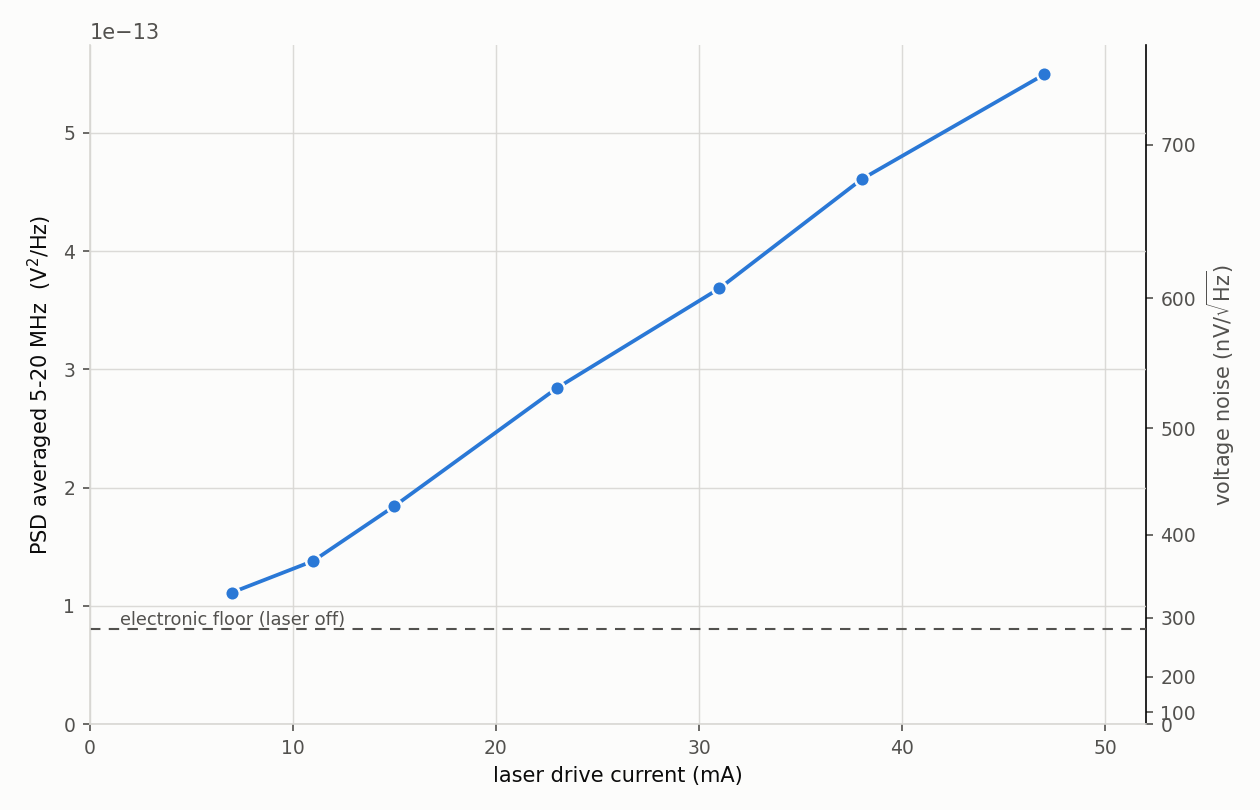
\includegraphics[width=1\linewidth]{psd_vs_current.png}
    \caption{5 - 20MHz Average PSD vs Laser Current with Balanced Detection}
    \label{fig:A2PSDvsCurrent}
\end{figure}

It can clearly be seen in \autoref{fig:A2PSDvsCurrent} and \autoref{fig:A2PSD} that the shot-noise exceeds the electronic noise floor at even the lowest measured laser currents, thus making the system shot-noise limited. As the current is increased, the system approaches the ideal shot-noise limit, as shot noise increasingly swamps out the electronic noise floor. 

Performance requirement P2 in \autoref{tab:requirements} requires that the total detector noise is within 1dB of the shot-noise limit. This requirement can be decomposed as follows:

Noise power adds in linear units, so letting $S$ be shot noise, and $E$ be every other noise source present here (electronic noise and any remaining RIN), the total noise floor, $T$ is given by:
\begin{equation}
    T = S + E = S(1+\frac{E}{S})
\end{equation}

Converting to dB:

\begin{equation}
    10log_{10}(S(1+\frac{E}{S}))=10log_{10}(S) + 10log_{10}(1 + \frac{E}{S})
\end{equation}
In this form, it can clearly be seen that as $S$ increases, the effect of $E$ on the total noise floor is increasingly reduced, as the second term, $10log_{10}(1+\frac{E}{S})$ approaches zero. This second term is the excess noise above the ideal shot-noise limit, which is given by $10log_{10}(S)$. Thus, in order to obtain a total noise floor which is within 1dB of the shot noise limit, we set:

\begin{equation}
    10log_{10}(1+\frac{E}{S})=1dB
\end{equation}
\begin{equation}
    \xrightarrow{}\frac{E}{S}\leq0.26
    \label{eqn:A2Crossover}
\end{equation}

Substituting the obtained electronic noise floor obtained in A1 into \autoref{eqn:A2Crossover}, we obtain:

\begin{equation}
    S \geq 3.1 \times 10^{-13}V^2/Hz
\end{equation}

Noting that \autoref{fig:A2PSD} and \autoref{fig:A2PSDvsCurrent} both give the \textbf{total} detector noise floor (shot \textbf{and} electronic noise), we require the total noise to be above $3.906 \times 10^{-13}V^2/Hz$ to gives a shot noise value of $3.1 \times 10^{-13}V^2/Hz$. This can be seen to be reached at a laser current of approximately 32mA. Above 32mA, the total detector noise floor is within 1dB of the ideal shot-noise limit, and the ideal shot-noise limit is further approached as the current is increased. 

From this, it can be seen that an operating current of 48mA for the laser allows P2 in \autoref{tab:requirements} to be met with the highest margin, and this will thus be used as the laser current for the remainder of this project. While a higher laser current still may be used, to even further approach the ideal shot-noise limit, this risks saturating the detector. The detector has a maximum incident power rating of 1.5mW on each photodiode \cite{detector  datasheet}. From the laser datasheet \cite{laser datasheet}, a current of 48mA gives approximately 17mW at the laser output, which will result in approximately 0.85mW at each detector from the LO alone. This allows the detector to thus remain comfortably far away from its saturation point, even if returned signal is high and results in a higher incident power at the photodiode after mixing with the LO. 

\subsubsection{A3: Relative Intensity Noise}
Experiment A3 serves only for completeness, to illustrate the effectiveness of balanced detection in removing relative intensity noise at the detector output. It was found that indeed 0.6125dB of RIN was cancelled by using the balanced detection setup. See Appendix \ref{appendix:RINValidation} for the full results and discussion of this supplementary experiment.  

\section{B: Phase-induced Intensity Noise}
\subsection{Experimental Goals}
As discussed in \autoref{sec:lit-noiseSources}, and elaborated in Appendix \ref{appendix:PIIN}, Phase-induced Intensity Noise (PIIN) can be a significant contributor to the total noise of the system, rising far above shot-noise - particularly when the linewidth of the laser source is not narrow, and when there is significant path-length mismatch between the LO and the transmit signal.

 The goal of Experiment B is to measure and quantify the magnitude and shape of the total noise of the system, including PIIN, in a controlled setting. There is effectively no target in this experiment, thus making all PIIN in the measurement attributable to reflections from the circulator and collimator, and independent of target. 
 
 
 \subsection{Experimental Methodology}
 For this experiment, the system is set up in full, as given by the final design in \autoref{fig:finalDesign}. The collimator is then pointed at a stationary matte-black painted surface, angled 45 degrees away from the collimator, and at a distance of 10cm from the collimator. Any reflections from the target surface will not be Doppler shifted, because it is stationary - thus, if these reflections are sent back into the collimator, they will appear at the output as additional PIIN (see Appendix \ref{appendix:PIIN}). This setup thus intends to absorb and reflect a large amount of the emitted light \textbf{away} from the system, so that the measured PIIN can be attributed to only the internal reflections in the system from the collimator and circulator, which is independent of target. 
 
 The laser is then driven with a current of 48mA (the chosen operating point for LO power), and the same oscilloscope acquisition chain and post-processing chain (Welch PSD) as in experiment A is used to obtain the PIIN power. As discussed in \cite{jiang_performance_2019}, PIIN can vary drastically depending on temperature, or small disturbances in the system's fiber optics, thus this measurement is repeated 16 times over the course of an hour to account for such variations. The average noise power as well as the spread from these measurements can then be computed. 
 
 \subsection{Results and Discussion}
 \autoref{fig:psdpiin} below gives the averaged PSD of the obtained noise measurements, with the electronic noise floor and the total noise floor (excluding PIIN) from Experiment A2 given as reference. 
 
\begin{figure}[H]
	\centering
	\includegraphics[width=1\linewidth]{"../Data Acquisition/figures/psd_piin"}
	\caption{Experiment B: Total noise in the system, including PIIN}
	\label{fig:psdpiin}
\end{figure}

 It can be seen that the total noise is now significantly above that measured in A2, owing to the excess noise introduced by PIIN. It can also be seen that as expected, PIIN varied significantly between measurements. In the 5 - 20MHz band, the total excess noise was measured to be from 12.2 to 14.2dB above the A2 noise floor, for a given frequency. It can also be seen that this excess noise is not constant, and starts rolling off steeply from approximately 10MHz. The shape of the PIIN corresponds to the $L_c \gg \Delta L$ regime described in Appendix \ref{appendix:PIIN}, as it is a flat floor and does not contain a Lorentzian peak at baseband.
 
 From these results it is thus clear that in this system, PIIN dominates other noise sources by a large amount, especially at lower frequencies. It is thus the largest single noise contributor in the total SNR of the system when trying to measure a Doppler peak, and the system is therefore no longer shot-noise limited (the ideal case).  
 
 \subsection{Reducing PIIN}
 The experiments in \autoref{sec:functionalTesting} were performed using the system as is, with the PIIN-limited behaviour observed and described above. It was found that while the system could adequately detect the velocity of a hard-target, it did not have enough sensitivity to detect the velocity of a seeded air-flow, owing to the high noise floor from PIIN. It was thus decided that an attempt would be made to reduce PIIN, from the theory discussed in \autoref{sec:lit-noiseSources} and elaborated in Appendix \ref{appendix:PIIN}. Obtaining a narrower linewidth laser source is out of budget for this project, thus the only remaining option was to attempt to better match the fiber optic path length between the LO and the received signal. This allows the LO and the received signal to be more coherent in phase at the detector. This is because the travel-time for both will be closer matched, meaning that the phase of the laser will not have been able to "wander" by as much between the two signals.
 
 FC/APC fiber patch cords of varying lengths were obtained and inserted in between the 10\% splitter arm and the one arm of the 50:50 mixer, to effectively increase the LO path length, in an attempt to closer match the longer path length followed by the received signal (which traverses the collimator and free-space twice, in excess of the LO path). The PIIN of the system was measured for each length of patch-cable using the same methodology previously described, with 10 averages for each patch cable length. The results are given in \autoref{fig:psdpiinlengths}:
 
\begin{figure}
	\centering
	\includegraphics[width=1\linewidth]{"../Data Acquisition/figures/psd_piin_lengths"}
	\caption{Total noise in the system for different inserted patch-cable lengths}
	\label{fig:psdpiinlengths}
\end{figure}

It can be seen that 